%-----------------------------------LICENSE------------------------------------%
%   This file is part of tikz_figures.                                         %
%                                                                              %
%   tikz_figures is free software: you can redistribute it and/or              %
%   modify it it under the terms of the GNU General Public License as          %
%   published by the Free Software Foundation, either version 3 of the         %
%   License, or (at your option) any later version.                            %
%                                                                              %
%   tikz_figures is distributed in the hope that it will be useful,            %
%   but WITHOUT ANY WARRANTY; without even the implied warranty of             %
%   MERCHANTABILITY or FITNESS FOR A PARTICULAR PURPOSE.  See the              %
%   GNU General Public License for more details.                               %
%                                                                              %
%   You should have received a copy of the GNU General Public License along    %
%   with tikz_figures.  If not, see <https://www.gnu.org/licenses/>.           %
%------------------------------------------------------------------------------%

% Use the standalone class for displaying the tikz image on a small PDF.
\documentclass[crop, tikz]{standalone}

% Import the tikz package to use for the drawing.
\usepackage{tikz}

% Begin the document.
\begin{document}

    % Draw the figure.
    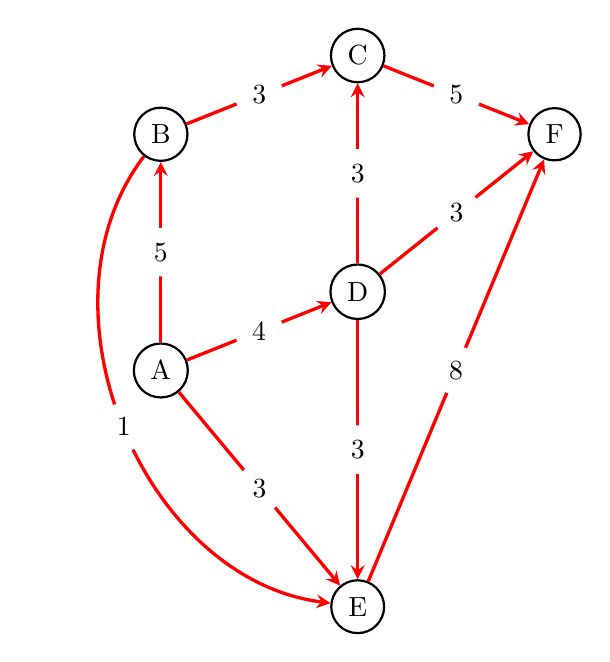
\begin{tikzpicture}
        \begin{scope}[%
            every node/.style = {%
                circle,
                thick,
                draw
            }
        ]

            % Nodes (vertices) of the graph.
            \node (A) at (0.0, 0.0) {A};
            \node (B) at (0.0, 3.0) {B};
            \node (C) at (2.5, 4.0) {C};
            \node (D) at (2.5, 1.0) {D};
            \node (E) at (2.5, -3.0) {E};
            \node (F) at (5.0, 3.0) {F};
        \end{scope}

        \begin{scope}[%
            > = stealth,
            every node/.style = {%
                fill = white,
                circle
            },
            every edge/.style = {%
                draw = red,
                very thick
            }
        ]

            % Edges of the graph.
            \path [->] (A) edge node {$5$} (B);
            \path [->] (B) edge node {$3$} (C);
            \path [->] (A) edge node {$4$} (D);
            \path [->] (D) edge node {$3$} (C);
            \path [->] (A) edge node {$3$} (E);
            \path [->] (D) edge node {$3$} (E);
            \path [->] (D) edge node {$3$} (F);
            \path [->] (C) edge node {$5$} (F);
            \path [->] (E) edge node {$8$} (F); 
            \path [->] (B) edge[bend right = 60] node {$1$} (E); 
        \end{scope}
    \end{tikzpicture}
\end{document}
